\newpage
\section{42. 接雨水}
\label{leetcode:42}

\subsection{题目}

给定 n 个非负整数表示每个宽度为 1 的柱子的高度图,
计算按此排列的柱子,下雨之后能接多少雨水。

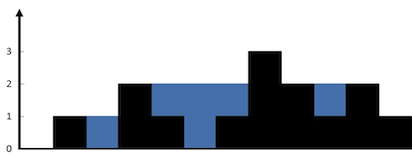
\includegraphics[width=100mm,height=50mm]{images/leetcode/rainwatertrap.png}

上面是由数组 [0,1,0,2,1,0,1,3,2,1,2,1] 表示的高度图,
在这种情况下,可以接 6 个单位的雨水(蓝色部分表示雨水)。\textbf{感谢 Marcos} 贡献此图。

\textbf{示例}:

\begin{verbatim}
  输入: [0,1,0,2,1,0,1,3,2,1,2,1]
  输出: 6
\end{verbatim}

\subsection{参考题解,栈}

用栈保存一个下降的序列。

\begin{verbatim}
/**
 * @param {number[]} height
 * @return {number}
 */
var trap = function(height) {
  var peek = function(stack) { return stack[stack.length - 1]; };
  let result = 0;
  let stack = [];
  for (let i = 0; i < height.length; i += 1) {
    while (stack.length > 0 && height[i] > height[peek(stack)]) {
      const top = stack.pop();
      if (stack.length === 0) {
        break;
      }
      let curWidth = i - peek(stack) - 1;
      let curHeight = Math.min(height[i], height[peek(stack)]) - height[top];
      let curArea = curWidth * curHeight;
      result += curArea;
    }
    stack.push(i);
  }
  return result;
};
\end{verbatim}
